\documentclass[twocolumn, 10pt]{article}

% ---------- Packages ----------
\usepackage[utf8]{inputenc}
\usepackage[T1]{fontenc}
\usepackage{times}
\usepackage{amsmath, amssymb}
\usepackage{enumitem}
\usepackage{graphicx}
\usepackage{titlesec}
\usepackage{setspace}
\usepackage{fancyhdr}
\usepackage{titling}
\usepackage{abstract}
\usepackage{wrapfig}
\usepackage[margin=1in]{geometry}
\usepackage{float}
\usepackage{booktabs}
\usepackage{caption}
\usepackage{parskip}
\usepackage{times}
\usepackage{hyperref}
\usepackage{titlesec}
\usepackage{listings}
\usepackage{xcolor}
\usepackage{mathtools}

% -------- Python Code ----------
\lstdefinestyle{mypython}{
  language=Python,
  basicstyle=\ttfamily\small,
  keywordstyle=\color{blue},
  commentstyle=\color{gray},
  stringstyle=\color{orange},
  showstringspaces=false,
  breaklines=true,
}

% --------- List Spacing --------
\setlist{itemsep=0.3em, topsep=0.5em}

% ---------- Geometry ----------
\geometry{
  top=0.9in,
  bottom=1in,
  left=0.9in,
  right=0.9in
}

% ---------- Header ----------
\pagestyle{fancy}
\fancyhf{}
\fancyhead[L]{Sebastian Newberry, Endri Islami, Parth Gajula}
\fancyhead[R]{April 28, 2025}
\renewcommand{\headrulewidth}{0.4pt}

% ---------- Title Customization ----------
\pretitle{\begin{center}\Large\bfseries\rule{\linewidth}{0.8pt}\\[0.5em]}
\posttitle{\\[0.5em]\rule{\linewidth}{0.8pt}\end{center}}
\preauthor{\begin{center}\normalsize}
\postauthor{\end{center}}
\predate{\begin{center}\small}
\postdate{\end{center}}

\title{Retrieval Augmented Generation – The Process of Improving Output Using External Resources}
\author{Sebastian Newberry \quad Endri Islami \quad Parthiv Gajula}
\date{April 28, 2025}

% ---------- Section Formatting ----------
\titleformat{\section}{\normalfont\Large\bfseries}{\thesection}{1em}{}
\titleformat{\subsection}{\normalfont\large\bfseries}{\thesubsection}{1em}{}
\titleformat{\subsubsection}{\normalfont\normalsize\bfseries}{\thesubsubsection}{1em}{}

% ---------- Document ----------
\begin{document}

\setlength{\abovedisplayskip}{6pt}
\setlength{\belowdisplayskip}{6pt}

\maketitle

\begin{abstract}
    Retrieval-Augmented Generation (RAG) is a framework that combines document retrieval with language generation to produce accurate, evidence-based responses. The process begins by retrieving documents relevant to a user query, which are then used to either extract exact answers or provide context for generation. As the size of the document corpus grows, retrieval becomes increasingly challenging. To address this, retrievers leverage document embeddings stored in vector databases to efficiently compute similarity scores between queries and documents. Advanced models, such as REALM, incorporate a reader component to re-rank retrieved documents based on relevance before passing them to a generator model like GPT. Other approaches, such as RETRO, integrate retrieved document chunks directly into the generation process using cross-attention, enabling tighter alignment between retrieval and generation. Although these methods share the common goal of improving factuality and relevance, they differ in their architectural choices and objectives. These objectives could be things like prioritizing retrieval accuracy, evidence extraction, or seamless integration with generation.
\end{abstract}

\section{Introduction}

The objective of this report is to develop a methodology for retrieving relevant information from a corpus of documents and either leveraging it alongside a generation model to produce accurate responses to user prompts, or finding an exact answer in a huge corpus of documents. Before delving into the detailed mechanics of both of these approaches, it is important to establish key terminology that will be referenced throughout the paper.

In the following sections, several important concepts will be defined. \textbf{Indexing} refers to the process of organizing and structuring document chunks to enable efficient retrieval. \textbf{Retrieval} denotes the method of selecting the most relevant documents from a larger collection based on a given query. A \textbf{reader} is defined as a model or algorithm that evaluates the relationship between a query and candidate documents. Finally, a \textbf{generator} is a model tasked with creating a coherent response using the information identified during retrieval and reading.

In retrieval systems, two primary encoder architectures are commonly utilized: the bi-encoder and the cross-encoder. A bi-encoder consists of two independently applied BERT models: one encodes the query and the other encodes candidate documents. Each input is processed separately, producing dense vector embeddings that capture the semantic content of either the query or the document. Relevance is then assessed by comparing these embeddings using similarity metrics such as Maximum Inner Product Search (MIPS) or Maximum Cosine Similarity (MCS).

In contrast, a cross-encoder jointly encodes the query and document by concatenating them and processing them together with a single BERT model. Self-attention is computed across both the query and document tokens, allowing for fine-grained interaction between them. A cross-encoder is typically trained to output a single relevance score indicating the degree of match between a query and a document. It can also be trained for more complex tasks, such as predicting the start and end token positions corresponding to an answer span within a document.

Although cross-encoders are highly effective at modeling fine-grained contextual similarities between queries and documents, they are computationally infeasible to use for large-scale retrieval. Evaluating a query against every document in a corpus would require running full self-attention across millions or billions of document-query pairs, which is prohibitively expensive in both time and computational resources. As a result, most retrieval systems rely on bi-encoder architectures for initial retrieval, sacrificing some fine-grained matching ability in exchange for scalability and efficiency.

\section{Literature Review}

The first significant research on Retrieval-Augmented Generation (RAG) was published in early 2020. During this period, much of the focus in the field was on developing algorithms capable of retrieving and ranking documents efficiently, while generation remained a secondary concern.

One of the earliest and most influential approaches was \textbf{REALM} (Retrieval-Augmented Language Model Pre-Training)~\cite{guu2020realm}. REALM employs a bi-encoder architecture, where queries and documents are embedded separately to facilitate efficient retrieval. A key contribution introduced by REALM was the formulation of retrieval as part of a probabilistic framework. Specifically, the probability of producing a correct output \( y \) given an input \( x \) is expressed by marginalizing over possible retrieved documents \( z \):
\begin{equation*}
p(y \mid x) = \sum_{z \in \mathcal{Z}} p(y \mid z, x) \, p(z \mid x)
\end{equation*}

REALM is specifically designed for tasks involving the identification of an exact answer span to a prompt within a document, predicting masked tokens, or finding additional context to be used for Open-Domain Question Answering (Open-QA). To support retrieval, REALM uses a bi-encoder-based \textbf{neural knowledge retriever}, embedding queries and documents separately. Both the query encoder and, optionally, the document encoder are trained during pretraining. Because updating the document encoder during training causes the document embeddings to become stale, REALM periodically re-embeds and re-indexes all documents every several hundred training steps to maintain retrieval consistency.

After retrieving the top-\(k\) documents for a query, a \textbf{knowledge-augmented encoder} is applied to each document separately. This reader model predicts a probability distribution over possible start and end positions for the answer span within each document. The final output is selected as the span with the highest predicted probability across all retrieved documents. For this component, REALM employs a cross-encoder architecture by concatenating the query and document, allowing the model to compute fine-grained contextual interactions between query and document passages.

Later in June and September 2020, two additional algorithms were developed to improve the retrieval component of retrieval-augmented generation frameworks. These algorithms are \textbf{ColBERT} (Contextualized Late Interaction over BERT) and \textbf{DPR} (Dense Passage Retrieval). Each provides a different approach to optimizing the retrieval probability \( p(z \mid x) \) within the RAG framework.

\textbf{DPR}~\cite{karpukhin2020dense} is designed to embed large passages into dense vector representations, which can then be efficiently stored and retrieved from a vector database. Compared to REALM, DPR introduces a key innovation: the use of contrastive learning to better supervise the retriever. In DPR, the model is trained to maximize the similarity between a query and its corresponding positive passage while minimizing similarity with negative passages. The paper introduces three methods for sampling negative passages during training:

\begin{itemize}
    \item \textbf{Random negatives:} Randomly selected passages that do not contain the correct answer.
    \item \textbf{BM25 negatives:} Top-ranked passages returned by a BM25 search that match many question tokens but do not contain the answer.
    \item \textbf{Gold negatives:} Passages that serve as positive examples for other questions in the training dataset.
\end{itemize}

\textbf{ColBERT}~\cite{khattab2020colbert} introduces a new approach to retrieval that differs from traditional dense retrievers. Like other retrieval algorithms, ColBERT uses a bi-encoder architecture where queries and documents are encoded separately using BERT. However, instead of pooling document or query representations into a single vector, ColBERT preserves token-level embeddings for both queries and documents. 

Each document token is independently encoded and stored in a compressed vector index. At retrieval time, each query token is encoded separately, and the similarity between a query and a document is computed through a late interaction mechanism. Specifically, for each query token, the maximum similarity with any document token is computed, and the overall score is the product of these maximum similarities:
\begin{equation*}
S_{q,d} := \prod_{i \in [|E_q|]} \max_{j \in [|E_d|]} E_{q_i} \cdot E_{d_j}
\end{equation*}
Unlike traditional cross-encoders that jointly attend over both queries and documents, ColBERT focuses on independent token-level matching. While this design allows for highly efficient retrieval over lots of tokens, it also means that ColBERT captures token-level relevance without modeling full cross-token contextualization between the query and document.
This means that ColBERT can be bad at understanding context of a sentence and instead often times only understands the meaning of tokens in documents but not exactly the entire context they are used in.

ColBERT also uses the same contrastive learning that DPR uses. ColBERT built on this contrastive learning by using relevance guided supervision. ~\cite{khattab2021relevance} This method is intended to solve the problem of finding negative samples to compare against when training ColBERT.
It works by finding negative samples in an initial ColBERT model with a sparse vector retrieval algorithm like BM25, then once the ColBERT retriever gets trained once, a new retriever is created that bases its negative samples off of the previous trained retriever.
In other words, after a certain batch of samples, a ColBERT retriever model will learn the bad samples, then a new ColBERT retriever will be created that uses the previous, partially trained retriever to find negative samples.

\begin{figure}[H]
    \centering
    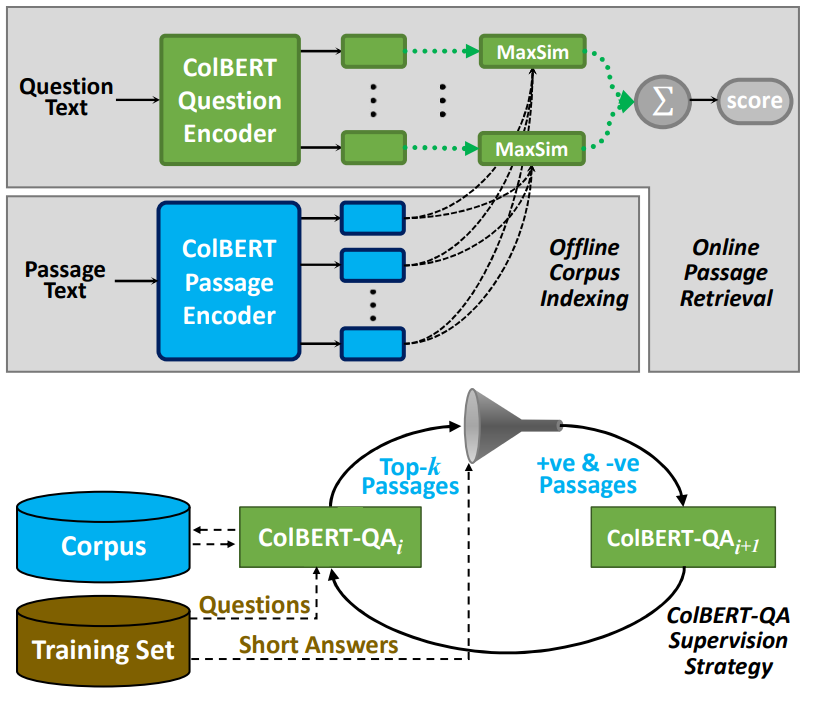
\includegraphics[width=0.5\linewidth]{ColBERT_OpenQA.png}
    \caption{Top: This figure showcases ColBERT token-by-token similarity search across all documents one query token at a time. Bottom: This figure shows ColBERT retrievers being trained based on negative samples coming from previous retrievers.}
    \label{fig:indexing-process}
\end{figure}

In April 2021, a model designed to both retrieve and generate text was developed. This model was \textbf{RAG} and was developed by Meta ~\cite{lewis2021retrieval}. Meta came up with two methods to effectively compute loss for retrieving documents based on queries, and generating text to answer a prompt. This model uses a BART encoder-decoder in order to both interpret context in documents for re-ranking,
and generate a unique answer based on the context that is passed to the BART encoder through cross-attention. The model also uses a DPR retriever that can be trained or already pre-trained.
\begin{itemize}
    \item \textbf{RAG-Sequence:} Uses the same retrieved documents to generate a complete sequence. Doesn't re-rank the top-k documents. Creates the entire probability distribution of an entire sequence coming out of all documents. Then multiplies that with the probability of the generator coming up with the correct token using the previous tokens and selected document. A summation is then taken over all tokens.
    \item \textbf{RAG-Token:} Uses the same retrieved documents to generate the complete sequence, but it does re-rank the top-k documents for every token. Re-creates a probability distribution of relevant documents for every token that gets generated. This then gets multiplied by the probability of generating the correct subsequent token based on previous tokens and the selected document. The summation comes first in this model, then the product to find the probability to generate the entire correct sequence comes afterwards because every token probability is found independently from one another.
\end{itemize}

Later in February 2022, research for another generation model came out. This model is called \textbf{RETRO} (Retrieval Enhanced Transformer) ~\cite{borgeaud2022improving}. This model separates an input into chunks, and fetches appropriate top-k documents for each chunk. It uses the traditional bi-encoder architecture to retrieve documents, then passes the original query through a self-attention layer to learn context, then the documents through cross-attention with the learned query embeddings to
an autoregressive decoder. This part of the process is called chunked cross attention. During chunked cross attention, subsequent tokens are generated only based on previous tokens just like a GPT model, but documents that were fetched from the previous chunk are used with cross attention. Cross attention occurs with the last token of the previous chunk and first 4 tokens of the next chunk in this specific implementation:

\begin{figure}[H]
    \centering
     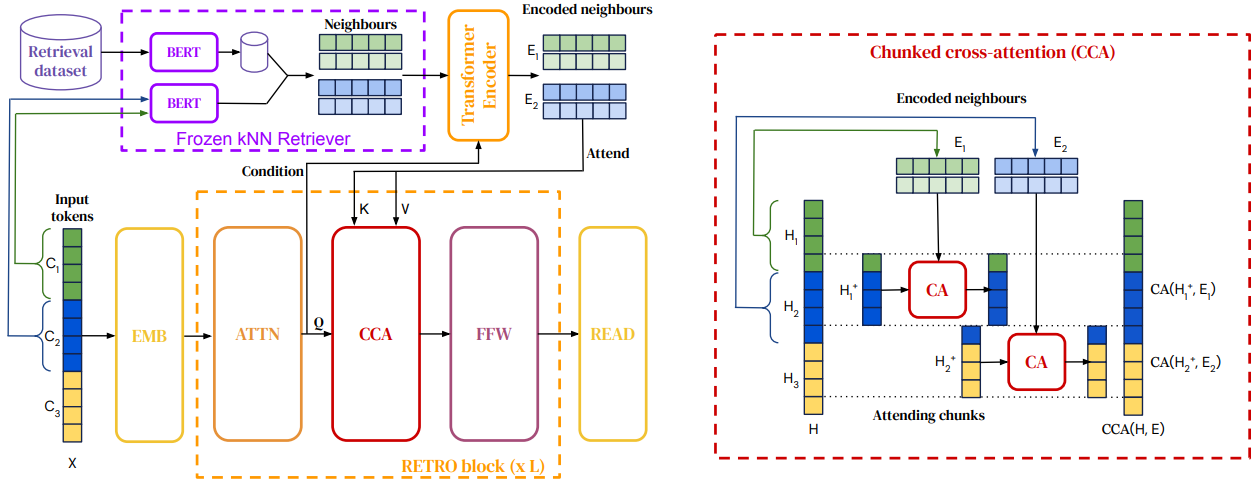
\includegraphics[width=\linewidth]{RETRO_CCA.png}
    \caption{Left: simplified version where a sequence of length \(n\) = 12 is split into \(l\) = 3 chunks of size \(m\) = 4. For each chunk, we retrieve \(k\) = 2 neighbours of \(r\) = 5 tokens each. Theretrieval pathway is shown on top. Right: Details of the interactions in the Cca operator. Causality is maintained as neighbours of the first chunk only affect the last token of the first chunk and tokens from the second chunk.}
    \label{fig:indexing-process}
\end{figure}

This version of crossed chunk attention allows for retrieving relevant documents, and also generating portions of text based on the next chunk of query tokens, along with documents that are relevant to the previous input.
One downside of RETRO is that it isn't compatible with pre-trained LLMs like LLAMA or GPT. In order to use it, the decoder part of this algorithm must be trained from scratch, and the retriever is typically pre-trained already, so only the generation portion of this algorithm is trained.

In August 2022, Meta developed Contriever~\cite{izacard2022unsupervised}, one of the first highly effective retrieval models that does not require labeled data to train.

Contriever is unique because it uses self-supervised contrastive learning to train itself without manually labeled positive or negative pairs. Instead, it applies a self-supervised denoising objective: given a document, two noisy views are created by randomly masking parts of the text. These two views are treated as a positive pair, while other documents in the batch serve as negatives.

During training, Contriever uses cosine similarity to measure how close two embeddings are. The model is trained with a contrastive loss that pulls together the positive pairs (high similarity) and pushes apart the negatives (low similarity).

Additionally, Contriever uses the same encoder for both queries and documents, unlike many earlier retrieval models that used separate encoders. Because it is not trained with domain-specific labels or tasks, Contriever remains highly domain-agnostic and adaptable to a wide variety of documents and retrieval tasks. It achieves state-of-the-art performance in zero-shot retrieval settings, where the model must retrieve relevant documents from domains it has never seen during training.

In December 2022, a model called \textbf{FiD} (Fusion-in-Decoder) was introduced to improve retrieval-augmented generation by more effectively leveraging multiple retrieved passages~\cite{deJong2022FiDO}.  
Instead of fusing passages early, FiD encodes each retrieved passage independently after prepending the query to each one.  
The encoder produces contextual embeddings for each (query, passage) pair separately.  
These encoded representations are then combined in the decoder, where cross-attention is performed over all encoded passages simultaneously to generate the output sequence.

In May 2023, an RAG implementation that contrasts RETRO was developed. This implementation is called \textbf{REPLUG} (Retrieve and Plug) ~\cite{shi2023replug}. The idea behind this is to use a pre-trained large language model, and treat the LLM as a black box. This means that the large language model is not trained.
The idea behind REPLUG is to train the retriever. In order to do this, two probability distributions are created. The first is the LLM probability that determines whether given an expected output and a query, how relevant is a document:
\begin{equation*}
Q(d \mid x, y) = \frac{e^{\text{PLM}(y \mid d, x) / \beta}}{\sum_{d' \in D'} e^{\text{PLM}(y \mid d', x) / \beta}}
\end{equation*}
Then another probability distribution is created, which finds that given a query, how relevant does the retriever think a document is:
\begin{equation*}
P_R(d \mid x) = \frac{e^{s(d,x)/\gamma}}{\sum_{d' \in D'} e^{s(d',x)/\gamma}}
\end{equation*}
Lastly, in order to train the retrieval, the loss function that is used is a KL divergence between these two distributions:
\begin{equation*}
\mathcal{L} = \frac{1}{|B|} \sum_{x \in B} \text{KL}\left( P_R(d \mid x) \, \| \, Q_{\text{LM}}(d \mid x, y) \right)
\end{equation*}
To put it simply, these equations are basically trusting that the LLM is correct in determining whether a specific document is relevant for a pair of inputs and outputs, and is using the output of the LLM to generate a loss for the retriever.


Lastly, In October 2023, research began shifting focus from merely optimizing retrieval algorithms to empowering large language models (LLMs) to decide when and how to use retrieved documents.  
\textbf{SELF-RAG} was introduced to address this new objective~\cite{asai2023selfrag}.  
SELF-RAG extends traditional retrieval-augmented generation by adding a self-reflection mechanism: the model not only generates the next token but also predicts auxiliary signals indicating its use of retrieved documents.  
Training combines standard language modeling objectives with additional self-supervised signals, without requiring human-annotated labels.

Specifically, the model predicts three types of auxiliary critique signals during decoding:

\begin{itemize}
    \item \textbf{isREL:} Whether the retrieved document is relevant to the input prompt.
    \item \textbf{isSUPP:} Whether the retrieved document supports the model's generated output.
    \item \textbf{isUSE:} Whether the model actually uses the document during generation.
\end{itemize}

During decoding, the model simultaneously predicts both the next token and the critique signals.  
The scoring function for each token combines the generation probability and a critique-based score:

\begin{equation*}
f(y_t, d, \mathcal{C}) = p(y_t \mid x, d, y_{<t}) + S(\mathcal{C})
\end{equation*}

where the critique score \(S(\mathcal{C})\) is defined as:

\begin{equation*}
S(\mathcal{C}) = \sum_{G \in \mathcal{G}} w_G \, s^G_t \quad \text{for} \quad \mathcal{G} = \{ \text{ISREL}, \text{ISSUP}, \text{ISUSE} \}
\end{equation*}

The model is trained to maximize the expected joint likelihood of generating correct outputs and accurate critique predictions:

\begin{equation*}
\max_{M} \mathbb{E}_{(x, y, r) \sim \mathcal{D}_{\text{gen}}} \left[ \log p_{M}(y, r \mid x) \right]
\end{equation*}

Correct predictions of the isREL, isSUPP, and isUSE signals lead to a lower loss, encouraging the model to appropriately incorporate retrieved information.  
Incorrect predictions result in a higher loss, discouraging reliance on irrelevant or unsupportive documents.

\section{Problem Statement}
The objective of Retrieval-Augmented Generation (RAG) to generate accurate outputs by leveraging external knowledge retrieved from a large corpus of documents can be mathematically expressed by marginalizing over the possible retrieved documents \( z \) as shown in the equation in the previous section:
\begin{equation*}
p(y \mid x) = \sum_{z \in \mathcal{Z}} p(y \mid z, x) \, p(z \mid x)
\end{equation*}
Here, \( p(z \mid x) \) denotes the probability of retrieving a relevant document \( z \) given the input \( x \), while \( p(y \mid z, x) \) denotes the probability of generating the correct output \( y \) conditioned on both the input and the retrieved document. This formulation separates the retrieval and generation components of the RAG pipeline and emphasizes the importance of jointly optimizing both stages to maximize overall performance.

In practice, retrieval models aim to maximize \( p(z \mid x) \) by selecting the most relevant documents from a corpus, while generation models aim to maximize \( p(y \mid z, x) \) by producing accurate and contextually appropriate outputs based on the retrieved information.

RAG introduces new optimization objectives by combining dense retrieval with autoregressive generation.  
For the \textbf{RAG-Sequence} model, a fixed set of top-k documents is retrieved once based on the input query. The model then generates an entire output sequence conditioned on each document independently, and marginalizes over documents after modeling the full sequence probability:
\begin{equation*}
p_{\text{RAG-Sequence}}(y \mid x) \approx \sum_{z \in \text{top-k}(p(\cdot \mid x))} p_{\eta}(z \mid x) \prod_{i=1}^{N} p_{\theta}(y_i \mid x, z, y_{1:i-1})
\end{equation*}
In the \textbf{RAG-Token} model, the same set of retrieved documents is used, but document contributions are dynamically re-weighted at each token generation step. This leads to a different loss formulation where marginalization over documents occurs independently for each token:
\begin{equation*}
p_{\text{RAG-Token}}(y \mid x) \approx \prod_{i=1}^{N} \sum_{z \in \text{top-k}(p(\cdot \mid x))} p_{\eta}(z \mid x) \, p_{\theta}(y_i \mid x, z, y_{1:i-1})
\end{equation*}
As a result, the summation over documents occurs inside the product over tokens in RAG-Token, whereas it occurs outside in RAG-Sequence.


Additionally, contrastive loss is used extensively in many of the retrieval methods defined above. The purpose of contrastive loss is to reduce similarity given to negative samples, and maximize similarity given to positive samples:

\begin{equation*}
\mathcal{L}(q, k^+) = -\frac{ \exp\left( s(q, k^+) / \tau \right) }{ \exp\left( s(q, k^+) / \tau \right) + \sum_{i=1}^{K} \exp\left( s(q, k_i) / \tau \right) }
\end{equation*}

Positive and negative samples can mean different things depending on the retrieval algorithm used. For the contriever, a positive sample is the same document that is masked with random noise, and a negative sample is a completely different document.
For ColBERT a negative sample is a specific document token embedding that doesn't match with a query token embedding, and a positive sample is one that does match. For DPR, a negative loss is a single passage in a document that doesn't match with the entire
query contextual embedding.
\section{Evaluation Method}

\subsection{Indexing}
Indexing is a foundational step in the Retrieval-Augmented Generation (RAG) pipeline, responsible for transforming raw data into a structured format suitable for efficient retrieval. It begins by extracting and cleaning documents from varied formats—such as PDF, HTML, and Markdown—into plain text. To accommodate the limited context windows of language models, the text is segmented into smaller, semantically meaningful chunks. These chunks are then embedded into vector representations using an embedding model and stored in a vector database for fast similarity-based retrieval during inference (Gao et al.).
\begin{figure}[H]
    \centering
     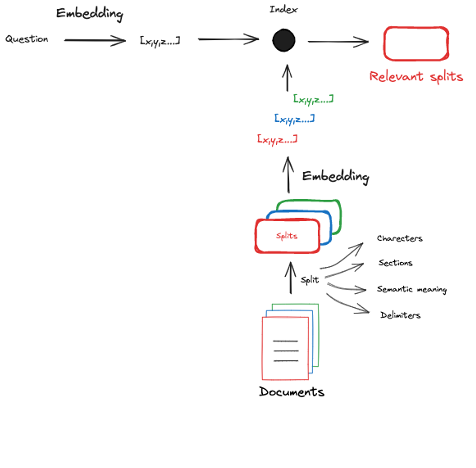
\includegraphics[width=0.5\linewidth]{firstimage.jpg}
    \caption{}
    \label{fig:indexing-process}
\end{figure}


\subsection{Splitting}

Splitting is a foundational step in the indexing pipeline of Retrieval-Augmented Generation (RAG) systems. It addresses a critical challenge in processing long-form documents—how to preserve semantic meaning while conforming to input length constraints of downstream models. The goal is to divide documents into manageable, semantically coherent chunks that can later be embedded as vector representations for retrieval.

\begin{figure}[H]
    \centering
    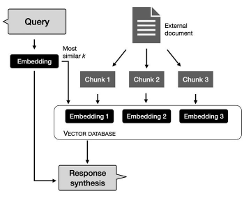
\includegraphics[width=\linewidth]{secondimage.jpg}
    \caption{}
    \label{fig:indexing-process}
\end{figure}


\subsubsection{Recursive Character-Based Splitting}

A widely adopted technique is the \texttt{RecursiveCharacterTextSplitter}, as utilized in frameworks like LangChain. This approach operates by recursively splitting text based on a prioritized list of delimiters such as paragraph breaks (\texttt{\textbackslash n\textbackslash n}), single line breaks (\texttt{\textbackslash n}), spaces (\texttt{ }), and finally, at the character level. This recursive logic ensures that the largest possible semantically coherent units are preserved while still adhering to predefined \texttt{chunk\_size} limits. 

For example, a chunk size of 1000 characters with an overlap of 200 characters is a common configuration to maintain continuity between adjacent chunks.

\begin{lstlisting}[style=mypython]
# Split Documents
text_splitter = RecursiveCharacterTextSplitter(
    chunk_size=1000, chunk_overlap=200
)

splits = text_splitter.split_documents(docs)
# Now `docs` contains chunks of text that are ready for embedding and indexing
\end{lstlisting}

This method ensures that important semantic boundaries, such as paragraph or sentence breaks, are respected as much as possible before falling back to more aggressive splitting criteria. As demonstrated in LangChain’s \textit{rag-from-scratch} repository, this process results in chunks that are better suited for embedding and semantic search tasks.


\subsubsection{Token-Aware Chunking with Overlap}

Another popular strategy is chunking by tokens, particularly with overlapping segments. Overlap is essential in preserving contextual information, especially for transformer-based models where the position of a token within its context heavily influences its representation. By ensuring that adjacent chunks share a fixed number of tokens—often referred to as a \textit{sliding window}—the model can capture cross-boundary semantics that might otherwise be lost. This method is particularly useful in scenarios where precision in retrieval is paramount, as it prevents fragmentation of key phrases or ideas that span multiple sentences.

\subsubsection{Structure-Aware Chunking}

More advanced methods adopt a \textbf{structure-aware strategy} that aligns chunks with syntactic units such as sentences or paragraphs. This is especially useful in tasks where fine-grained semantic relationships matter, such as question answering or summarization. In structure-aware models, small text units (e.g., a sentence) are treated as atomic retrieval elements, but their broader meaning is interpreted in the context of surrounding units. Thallys Costalat (2024) emphasizes that such methods yield higher retrieval precision, as the coherence of the chunk directly correlates with its informativeness during retrieval. Sentence-based chunking, for example, can be extended with ``context windows'' by appending neighboring sentences, creating composite chunks that balance granularity and context.



\subsection{Splitting Strategy Summary}

\begin{table}[H]
\centering
\begin{tabular}{|p{0.25\linewidth}|p{0.28\linewidth}|p{0.38\linewidth}|}
\hline
\textbf{Splitting Strategy} & \textbf{Key Feature} & \textbf{Use Case Scenario} \\
\hline
Recursive Character TextSplitter & Flexible-fallback through-delimiters & General-purpose chunking-of-large documents \\
\hline
TokenOverlap Chunking & Preserves continuity across segments & Semantic search with transformers-(e.g., BERT, GPT) \\
\hline
Structure-Aware Chunking & Aligns with linguistic structure & High-precision- retrieval or summarization tasks \\
\hline
\end{tabular}
\caption{}
\label{tab:splitting-strategies}
\end{table}



Each technique addresses a different trade-off between semantic preservation, context integrity, and chunk manageability. Selecting an appropriate method depends on the downstream task, document type, and retrieval sensitivity.

\subsection{Embedding}

After documents are split into semantically coherent chunks, the next stage in the RAG indexing pipeline is embedding, which transforms textual data into numerical vector representations. These embeddings allow for efficient semantic comparison, search, and retrieval within high-dimensional vector spaces.

\subsection{Purpose of Embedding}

Embedding serves as a bridge between unstructured textual information and structured numerical computation. By encoding each chunk into a dense vector, embedding models enable similarity comparisons based on vector proximity (e.g., cosine similarity or dot product), rather than relying solely on keyword overlap. This transformation is essential because it allows RAG systems to compare the semantic meaning of queries and documents, rather than just their surface-level lexical content.

\subsection{Types of Representations}

There are two principal methods for representing text:

\begin{itemize}
    \item \textbf{Statistical Representations:} Techniques like Bag-of-Words (BoW) and TF-IDF produce sparse vectors, which are simple but often fail to capture semantic nuance.
    \item \textbf{Machine-Learned Embeddings:} Transformer-based models like DPR (Dense Passage Retrieval), ColBERT, RAPTOR, and CONTRIEVER generate dense vectors, which embed semantic meaning into a compact numerical format suitable for neural retrieval methods.
\end{itemize}

\begin{figure}[H]
    \centering
   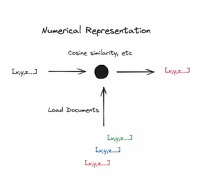
\includegraphics[width=0.85\linewidth]{thirdimage.jpg}
    \caption{}
    \label{fig:indexing-process}
\end{figure}



The latter is the standard in RAG systems due to its superior performance in understanding context, paraphrasing, and semantic similarity.

\begin{figure}[H]
    \centering
    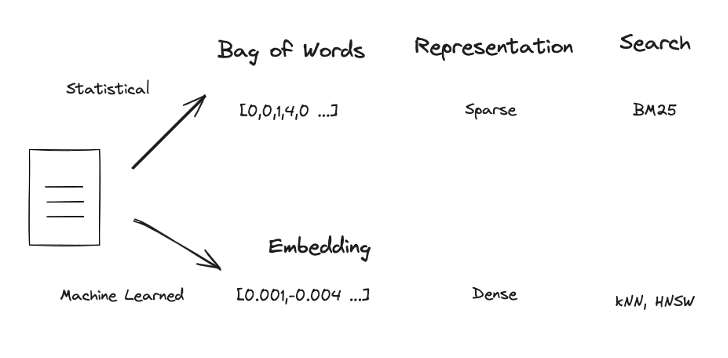
\includegraphics[width=\linewidth]{fourthimage.jpg}
    \caption{}
    \label{fig:indexing-process}
\end{figure}

\subsection{Common Embedding Models}

\begin{itemize}
    \item \textbf{DPR:} Generates a single vector per passage, optimized for full-document semantic similarity.
    \item \textbf{ColBERT:} Computes token-level embeddings, allowing fine-grained interaction between queries and passages, ideal for high-resolution retrieval.
    \item \textbf{RAPTOR:} Leverages hierarchical encoding and retrieval patterns for multi-hop reasoning.
    \item \textbf{CONTRIEVER:} Focuses on unsupervised learning of sentence-level representations, suitable for low-resource or domain-adaptive scenarios.
\end{itemize}

\subsection{Embedding Challenges}

\begin{enumerate}
    \item \textbf{High Dimensionality:} Embedding vectors typically exist in hundreds or thousands of dimensions. Searching or comparing vectors in such high-dimensional spaces is computationally intensive. Classical structures like KD-trees degrade rapidly beyond 10 dimensions.
    
    \item \textbf{Approximate vs. Exact Search:}
    \begin{itemize}
        \item \textbf{Exact Nearest Neighbor Search} guarantees precision but scales poorly.
        \item \textbf{Approximate Nearest Neighbor Search (ANNS)}—as used in libraries like FAISS—sacrifices some accuracy for speed and scalability. Tuning these systems is non-trivial and often domain-specific.
    \end{itemize}
    
    \item \textbf{Incompatible Representations:} 
    Not all embeddings are interoperable. For instance:
    \begin{itemize}
        \item \textbf{ColBERT} produces embeddings at the token level, optimized for fine-grained matching.
        \item \textbf{DPR} represents entire passages with a single embedding.
    \end{itemize}
    These differences mean that one cannot interchangeably use embeddings from different models within the same vector store. Each embedding model encodes information at a different granularity and semantic level, affecting retrieval performance and indexing compatibility.
\end{enumerate}

\subsection*{Embedding Models Comparison}

\begin{table}[H]
\centering
\begin{tabular}{|p{0.22\linewidth}|p{0.22\linewidth}|p{0.22\linewidth}|p{0.28\linewidth}|}
\hline
\textbf{Model} & \textbf{Granularity} & \textbf{Search Type} & \textbf{Use Case} \\
\hline
DPR & Passage-level & Dense vector search& General-purpose-retrieval \\
\hline
ColBERT & Token-level & Late interaction model& Fine-grained, high-precision retrieval \\
\hline
RAPTOR & Hierarchical & Hybrid & Multi-hop-or layered reasoning \\
\hline
CONTRIE-VER & Sentence-level & Dense unsupervised & Domain adaptation \\
\hline
\end{tabular}
\caption{}
\label{tab:embedding-models}
\end{table}

\section{Dataset Details}

\section{Experimental Results}

\section{Conclusion}

\bibliographystyle{plain}
\bibliography{references}

\end{document}